%% =====================================================================
%%  7 Discussion
%%  Interpretation of the answer: geometry, the control gap, model-form
%%  honesty, the latency budget, transferability. No new results.
%% =====================================================================
\section{Discussion}
\label{sec:discussion}

\subsection{Interpretation of the prediction}
\label{sec:disc-meaning}

At the adopted point the ball centre crosses \SI{0.9}{m} inside the right post
and \SI{0.5}{m} below the crossbar, in the upper-right third of the mouth as
the kicker sees it. The whole ball must pass inside the frame, so the
clearances to the post and the bar are \SI{0.77}{m} and \SI{0.38}{m}. In the elite sample of \citep{higueras2020} the mean lateral
position is \SIrange{2.27}{2.33}{m} and the upper third holds about a third of
the kicks, so the predicted point is a specific, moderately ambitious
placement \SI{0.4}{m} to \SI{0.5}{m} farther out than average.

The residual risk is asymmetric, and the asymmetry is a property of the adopted
model rather than of the earlier mixture: at the adopted \SI{5}{mm} noise
$0.0$\,\% of the draws finish wide of the post, $0.7$\,\%
pass over the bar and $2.1$\,\% clip the frame, the last group being
split between the post and the bar by the clearance test. Width is controlled: the
fixes pin the lateral coordinate early, and the envelope in $y$ is set by
model choice. Height is not, because the vertical acceleration is gravity,
which is known, plus a smaller aerodynamic term that the data constrain only
weakly, acting over the remaining \SI{0.3}{s} of flight with a lever arm of
$t^2/2$. A prediction that is approximately right in $y$ can therefore be
wrong in $z$ by tens of centimetres, comparable to the clearance under the bar
itself. The largest probability mass of a miss is therefore not at the posts
but above the goal.

\subsection{Origin of the control-model disagreement}
\label{sec:disc-disagreement}

The two controls in Section~\ref{sec:results} start from the same
six numbers and end \SI{0.53}{m} apart in $y$, while their heights agree to
about \SI{0.03}{m}. A lateral disagreement cannot come from flight time,
gravity or drag, and it is not a data error: both controls reproduce the
fixes. It is a statement about lateral force.

The identity is elementary. If the only forces are gravity and drag,
the aerodynamic force is antiparallel to the velocity, so the horizontal
velocity direction cannot change and the horizontal path is straight: the ball
crosses the plane at $y=11\,v_{0y}/v_{0x}$ exactly, for any drag coefficient.
The measured acceleration violates the identity. The fixes give
$a_y/a_x=1.00$, whereas a drag force acting on the velocity
$(30.4,\,9.4,\,6.9)$~m/s would give $a_y/a_x=v_{0y}/v_{0x}\approx0.31$; the
difference is a force perpendicular to the velocity. Drag can change the
flight time and hence the height at the plane, but it cannot move the crossing
sideways at all.

The two controls differ in how each supplies that force. The
constant-acceleration control, E1, extrapolates the lateral deceleration that
the fixes measure directly. The literature-prior Bayesian control, E2, cannot
do that without choosing a spin, so it fixes the transverse force from its prior
and lets the rest of the fit absorb the difference; its entry point is
displaced by whatever the prior supplies. The gap is therefore an indirect
measurement of the transverse force: the controls bracket its effect by making
opposite assumptions about it, the six-parameter fit frees the two coefficients
instead of assuming them, and the pair is quoted as a bracket, not as two
answers. Nor does the origin of the force matter: a ball
with little or no spin can be deflected sideways by an asymmetric wake, a
force comparable to the Magnus force \citep{texier2016}, so the fitted
coefficients absorb whichever mechanism is present.

\subsection{Calibration of the stated uncertainty}
\label{sec:disc-honesty}

Published inverse analyses solve the neighbouring problem. \citep{jsme2014}
recover the drag and lift coefficients of a sports ball from the shape of a
whole trajectory, using flight distance and maximum height or local curvature
and torsion; \citep{nathan2008pitchfx} recover drag, lift and the spin vector
of \num{99} tracked pitches. Both observe the curvature directly over the
whole flight. Our two fixes span
\SI{0.10}{s} of a \SI{0.40}{s} flight, with no observed spin. The coefficients
are then degenerate with the launch velocity; the deliverable cannot be a
parameter estimate, but the crossing point together with the range of crossings
that different model forms allow.

The calibration experiment exposes how much of that range is model error. With
\num{1000} synthetic truths drawn from a distribution that includes a vertical
Magnus component, the calibrated model's nominal \SI{90}{\percent} interval in $z$
covers only $0.446$ of them and has to be widened by $\lambda_z=4.94$, whereas the $y$
interval is almost correctly sized ($\lambda_y=0.96$). A factor near five is
not a numerical artefact: the profile and Wald widths of the $z$ interval
agree to \SI{0.6}{\percent}, so the interval is internally consistent and
still too narrow, because the fit omits a vertical force that the truths carry. That missing force is the same transverse force seen edge-on, which is
why an interval from any single model must not be read as a probability
statement about the height, and why the envelope, not the fitted posterior
interval, is the uncertainty statement of this paper: the envelope's $y$ range,
\SIrange{2.125}{3.121}{m}, is wider than any single model's interval and is
explicitly a model range. A probability statement is available only
conditional on a model; the envelope is the range that survives that choice. We
give both and label them.

\subsection{The latency budget}
\label{sec:disc-timing}
\begin{figure}[htbp]
  \centering
  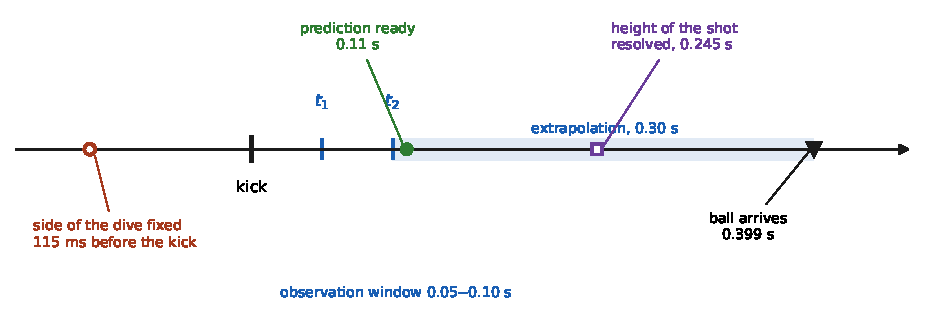
\includegraphics[width=0.90\textwidth]{f15-timeline.pdf}
  \caption{The prediction window against the two biological deadlines. The side
  of the dive is fixed about \SI{115}{ms} before the kick, so no post-kick
  measurement can change it; the height of the shot is resolved only about
  \SI{245}{ms} after contact. The estimate of this paper is ready at
  \SI{0.11}{s}, \SI{135}{ms} before the height becomes available to the
  goalkeeper and \SI{0.29}{s} before the ball arrives.}
  \label{fig:timeline}
\end{figure}


The two fixes arrive at \SI{0.10}{s}. Fitting the six parameters and
propagating their covariance costs about \SI{8}{ms} plus \SI{0.5}{ms} on one
core, so the estimate and its interval are ready roughly \SI{0.11}{s} after
the kick. The ball reaches the plane at
\SI{0.399}{s}. The biological deadline is different from what it is often taken
to be: goalkeepers commit to the \emph{side} about \SI{115}{ms} \emph{before}
the ball is struck, but they resolve the \emph{height} of the shot only about
\SI{245}{ms} \emph{after} contact \citep{higueras2020}. A prediction issued at
\SI{0.11}{s} therefore cannot change a decision that has already been taken a
tenth of a second earlier; what it supplies is the height and the arrival point,
\SI{135}{ms} before the keeper can extract that information from the flight
itself and \SI{0.29}{s} before the ball arrives. The value of the method is an
extrapolation of the transverse force over the remaining three quarters of the
flight, integrated from the first \SI{0.10}{s}, not a faster reaction.

The engineering budget belongs to the tracker rather than to the estimator.
Two three-dimensional positions to about a centimetre within \SI{0.10}{s} are
needed, from calibrated cameras. Goal-line technology already reaches
\SI{1.5}{cm}, but it is allowed a full second to report \citep{fifa2020glt},
and broadcast tracking systems are certified in two dimensions only
\citep{fifa2025epts}. The binding deadline is the keeper's \SI{245}{ms} height decision, not the
one-second reporting rule, and the prediction meets it with \SI{135}{ms} to
spare.

\subsection{Transferability}
\label{sec:disc-transfer}

The problem is not specific to football. Whenever a
projectile is observed only over a short early arc, the launch state and the
aerodynamic lift are nearly degenerate, and a point prediction is less honest
than a range. The same inverse problem appears in baseball, where tracked
pitches yield drag, lift and the spin vector \citep{nathan2008pitchfx}, and in
table tennis, where spin is inferred from the ball's flight
\citep{achterhold2023}. Two lessons transfer. First, report the range that
model choice allows, not only the interval that one model gives:
impact-point distributions computed from uncertain aerodynamic parameters have
non-Gaussian tails that a single-model interval hides
\citep{mehta2015,williamson2017}. Second, treat the observation design as part
of the inference, because a wider baseline or a direct spin measurement buys
more than a better estimator of the same two numbers \citep{shorter2013}. The
scope is the penalty flight, a \SI{0.4}{s} trajectory with an approximately
fixed spin axis and a uniform wind; beyond it the envelope should be
recomputed rather than rescaled.
